\chapter{METHODOLOGY}
{\baselineskip=2\baselineskip
	
This chapter presents the research methodology used in the study, it covers the in-depth details of the procedures and steps taken in the research design, design procedure, system development, and deployment process of this study.


\section {System Architecture} \label{Section 3.1}

\begin{figure}[h]
	\centering
	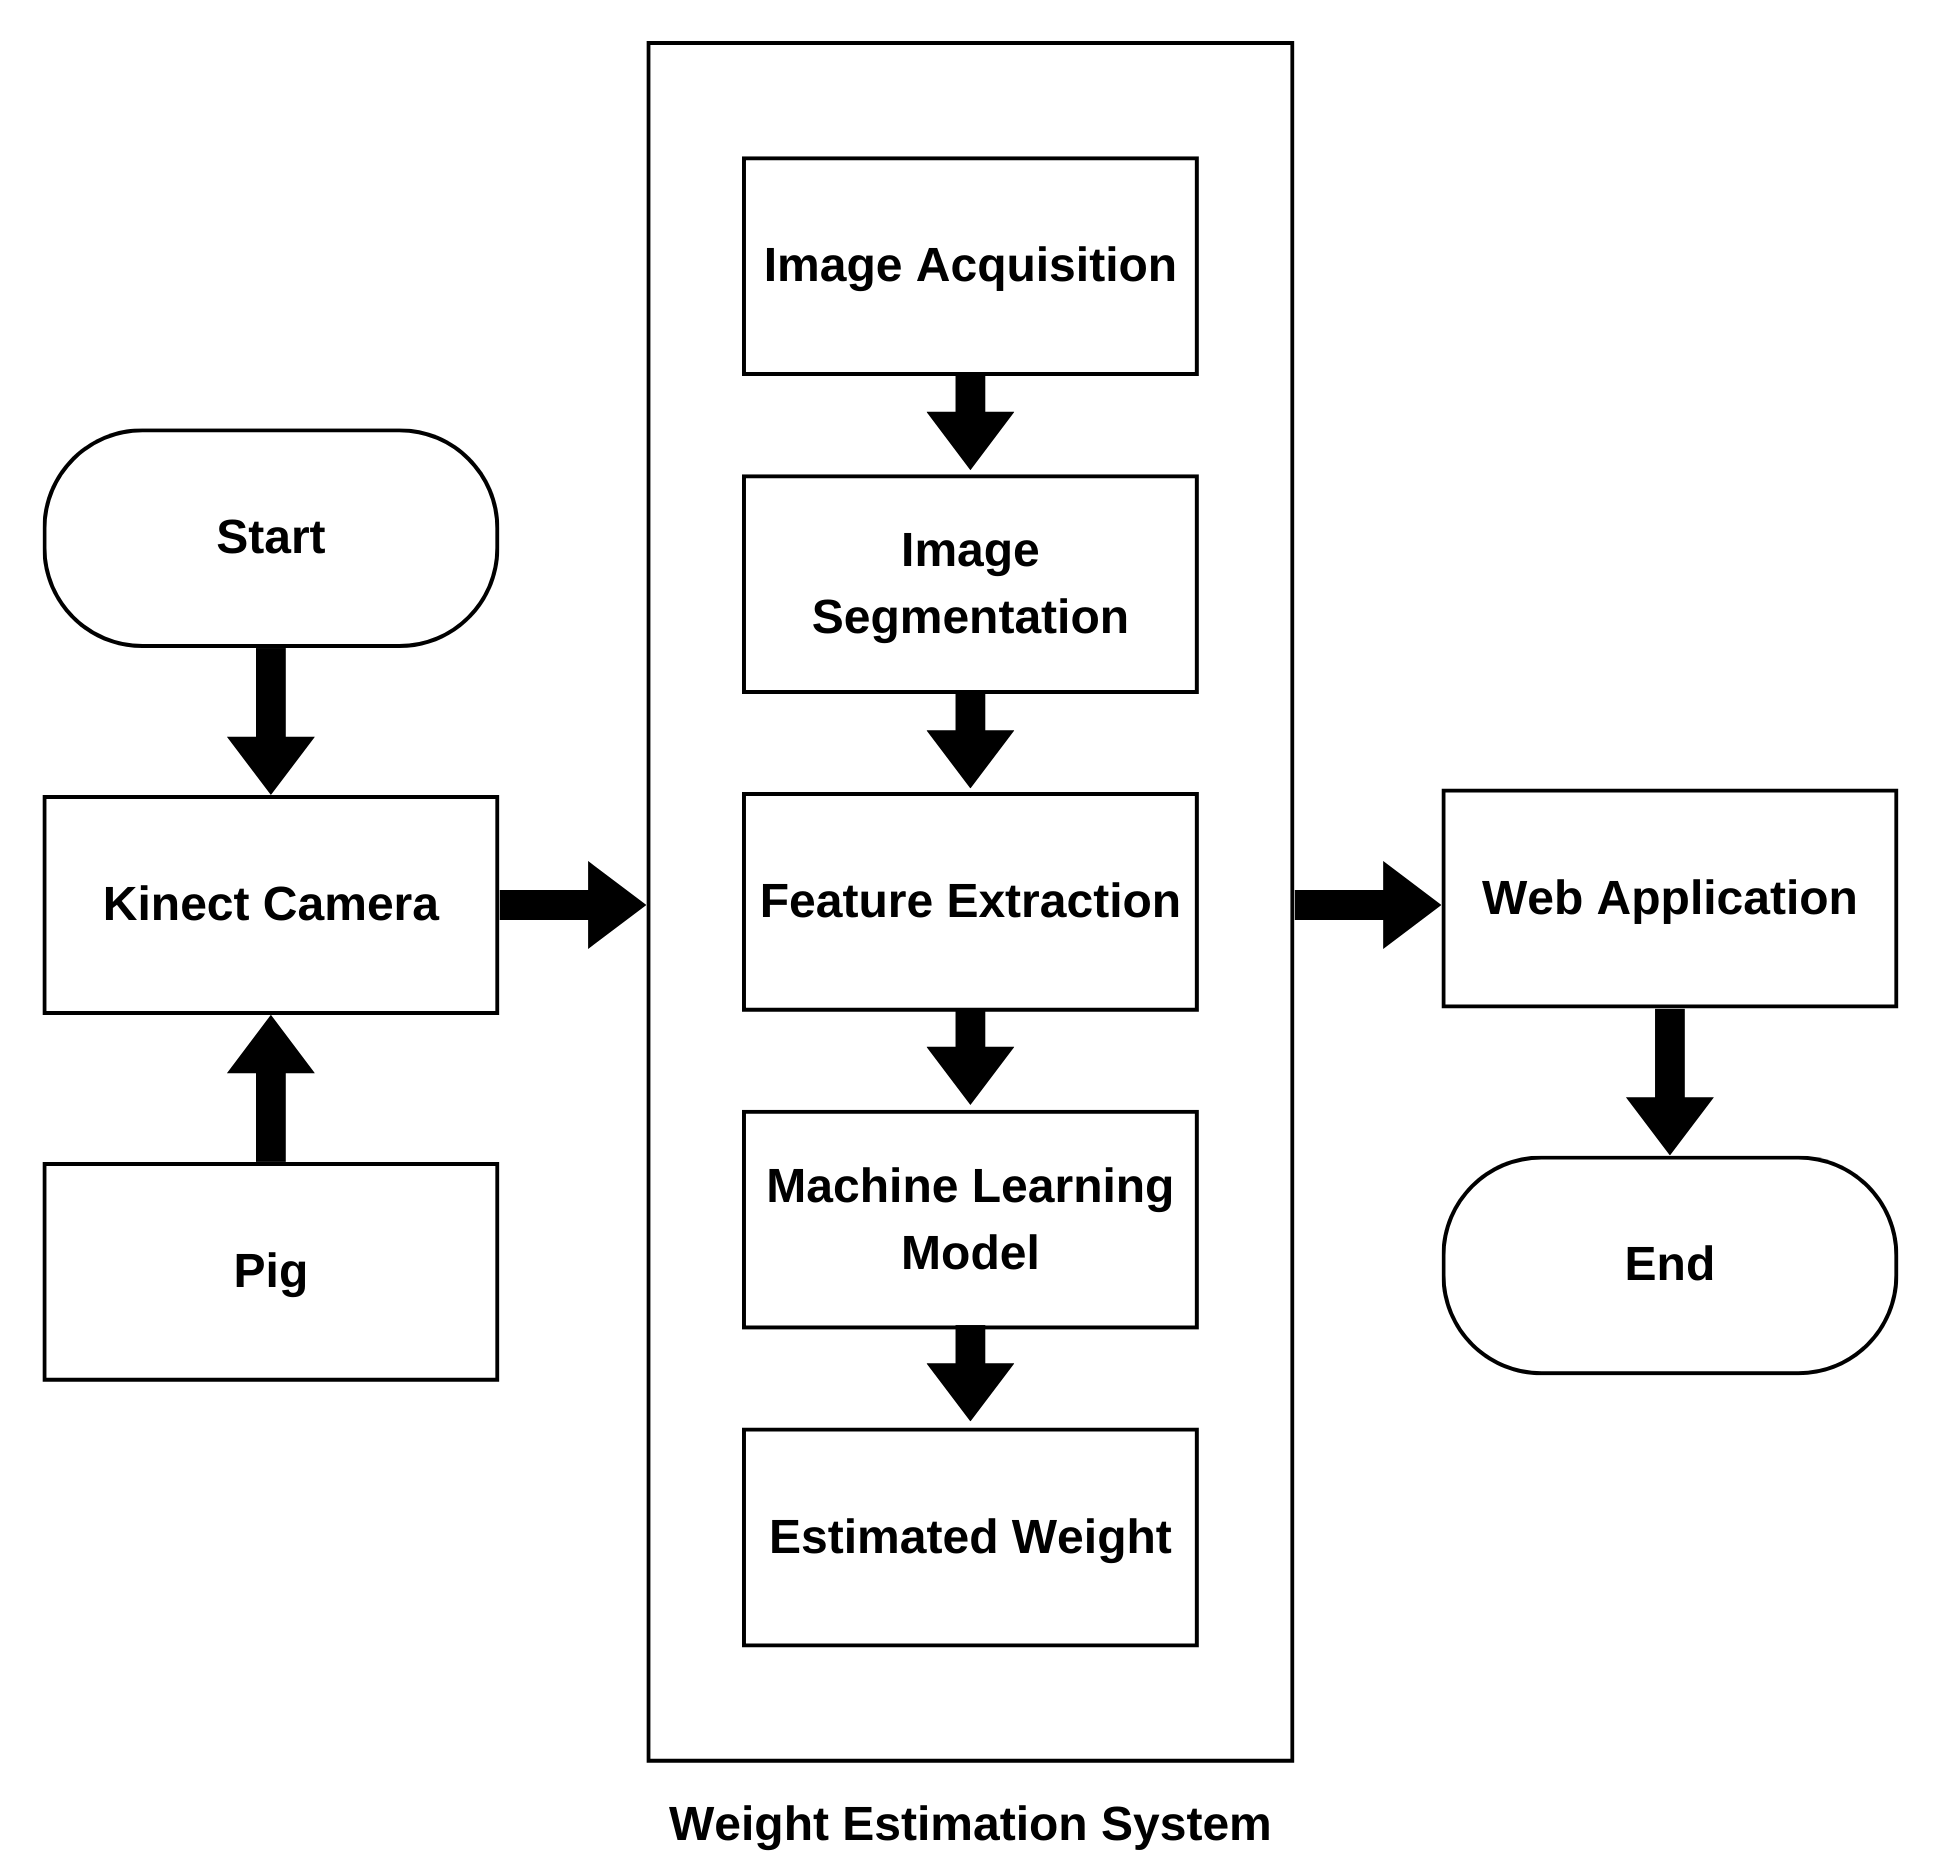
\includegraphics[height=0.5\textheight]{figures/Architectureofniggas}
	\caption{System Architecture}
	\label{fig:System Architecture}
\end{figure}

Figure 2 illustrates the system architecture of the pig weight estimation system. The system comprises the Landrace pig to be captured, the Microsoft Kinect V1 camera for acquiring depth and RGB images, and a processing system for data analysis. A laptop or dedicated server processes the data, performing image preprocessing, feature extraction (including 9 features such as pixel size, volume proxy, and sectional volumes), and weight estimation using a hybrid LightGBM-CNN model. The results are accessible through a FastAPI-based web service and a React-based web application, enabling real-time validation of actual and estimated weights. The architecture integrates hardware and software components, optimized for small-scale pig farms.

\subsection {Waterfall Model}
\begin{figure}[h]
	\centering
	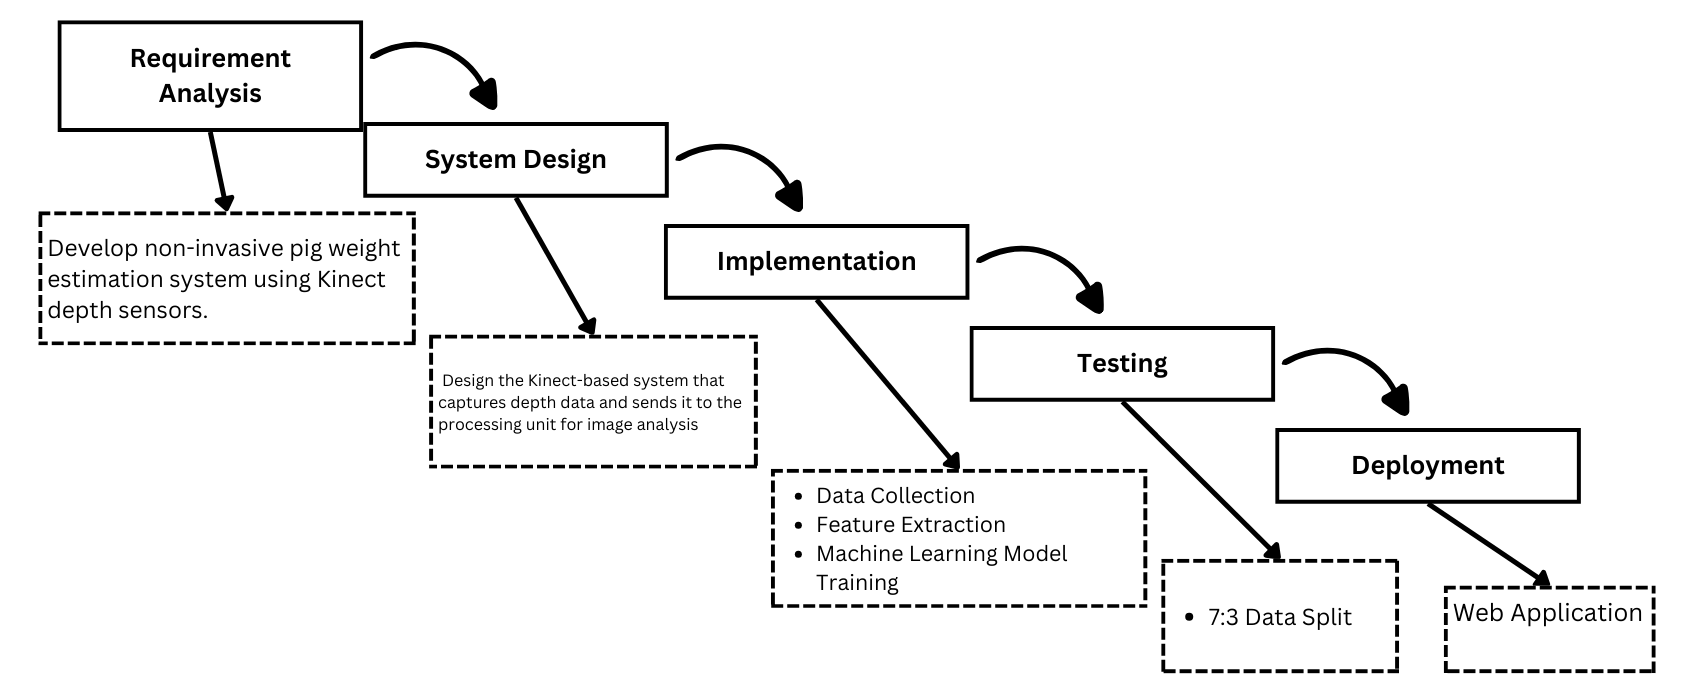
\includegraphics[height=0.3\textheight]{figures/Requirement Analysis (4)}
	\caption{Waterfall Model}
	\label{fig:Waterfall Model}
\end{figure}

Figure 3 depicts the Waterfall Model used for system development, following a linear, sequential approach:
\begin{itemize}
	\item \textbf{Requirement Analysis}: The goal is a non-invasive pig weight estimation system using a Kinect V1 depth sensor to capture depth images, extract 9 features \hyperref[Section 3.7]{(Section 3.7)}, and predict weight with a hybrid LightGBM-CNN model, accessible via a web application.
	\item \textbf{System Design}: The architecture includes hardware (Kinect V1, computer, pigpen) and software (YOLOv11, SAM, LightGBM-CNN, FastAPI, React) components, designed for compatibility and scalability.
	\item \textbf{Implementation}: Involves collecting depth and RGB images, extracting features, and training the hybrid model. Image processing includes grayscale conversion, contour detection, PCA-based alignment, and body part segmentation. The dataset follows an 80:20 training-validation split.
	\item \textbf{Testing}: Evaluates accuracy using Mean Absolute Error (MAE) and Root Mean Squared Error (RMSE) on a test set (20\% of data), selecting the most accurate model for deployment.
	\item \textbf{Deployment}: The system is deployed via a FastAPI web service and React web application on a local server, enabling real-time weight estimation.
\end{itemize}
The Waterfall Model ensures a structured development process with clear milestones.

\subsection {Flowchart}
\begin{figure}[h]
	\centering
	\includegraphics[height=0.45\textheight]{figures/Flowchart2Large}
	\caption{Flowchart}
	\label{fig:Flowchart}
\end{figure}

Figure 4 outlines the flowchart of the weight estimation system, detailing the end-to-end process from initialization to real-time weight prediction:
\begin{itemize}
	\item \textbf{System Initialization}: The Kinect V1 camera, computer system, and pigpen are powered on, and the pig is prepared for imaging. The camera is mounted at 1.9 meters, ensuring a clear top-down view of the pig’s back.
	\item \textbf{Realtime Video Capture}: The Kinect V1 captures synchronized RGB and depth video streams at 1280$\times$480 pixels, 30 frames per second, which translates to 30 images per second. A high-quality image is defined as clear, well-lit, free of motion blur, and accurately representing the pig’s dimensions without occlusion from other pigs.
	\item \textbf{Object Detection}: YOLOv11 processes the RGB stream to detect pigs, generating bounding boxes for each individual, which are mapped to the depth stream for accurate data extraction.
	\item \textbf{Segmentation}: The Segment Anything Model (SAM) isolates each pig within its bounding box, creating binary masks to remove background noise from the depth image.
	\item \textbf{Advanced Image Processing}: The depth image undergoes depth normalization, contrast enhancement, and optional data augmentation to enhance the quality and consistency of the image.
	\item \textbf{Feature Extraction}: Eleven features are extracted, including pixel size, non-zero pixel count, pixel-to-non-pixel ratio, standard deviation of depth, mean depth, pixel ratio, volume proxy, aspect ratio, and perimeter for each body part.
	\item \textbf{Preprocessing for Prediction}: Each of the 30 depth images extracted per second is resized to 40$\times$80 pixels, thresholded (values $\leq$1 set to 0), and normalized to [0, 1]. The mean of the features are taken, min-max normalized, and formatted for model input.
	\item \textbf{Weight Prediction}: The preprocessed depth image and features are sent to the FastAPI /predict/ endpoint. The LightGBM model processes the 9 features for an initial prediction, which is concatenated with CNN features (from the depth image) to produce the final weight prediction.
	\item \textbf{Result Display}: The predicted weight is returned via the FastAPI API and displayed on the React-based web application, showing the estimated weight alongside confidence indicators for user validation.
	\item \textbf{Iteration}: The process repeats for continuous real-time estimation, capturing new frames as pigs move within the pigpen, ensuring only high-quality frames are processed.
\end{itemize}
The flowchart ensures a robust, automated pipeline for real-time weight estimation, integrating seamlessly with the deployed system.

\section{Experimental Setup}

\newpage

\subsection {Pigpen Diagram}

\begin{figure}[h]
	\centering
	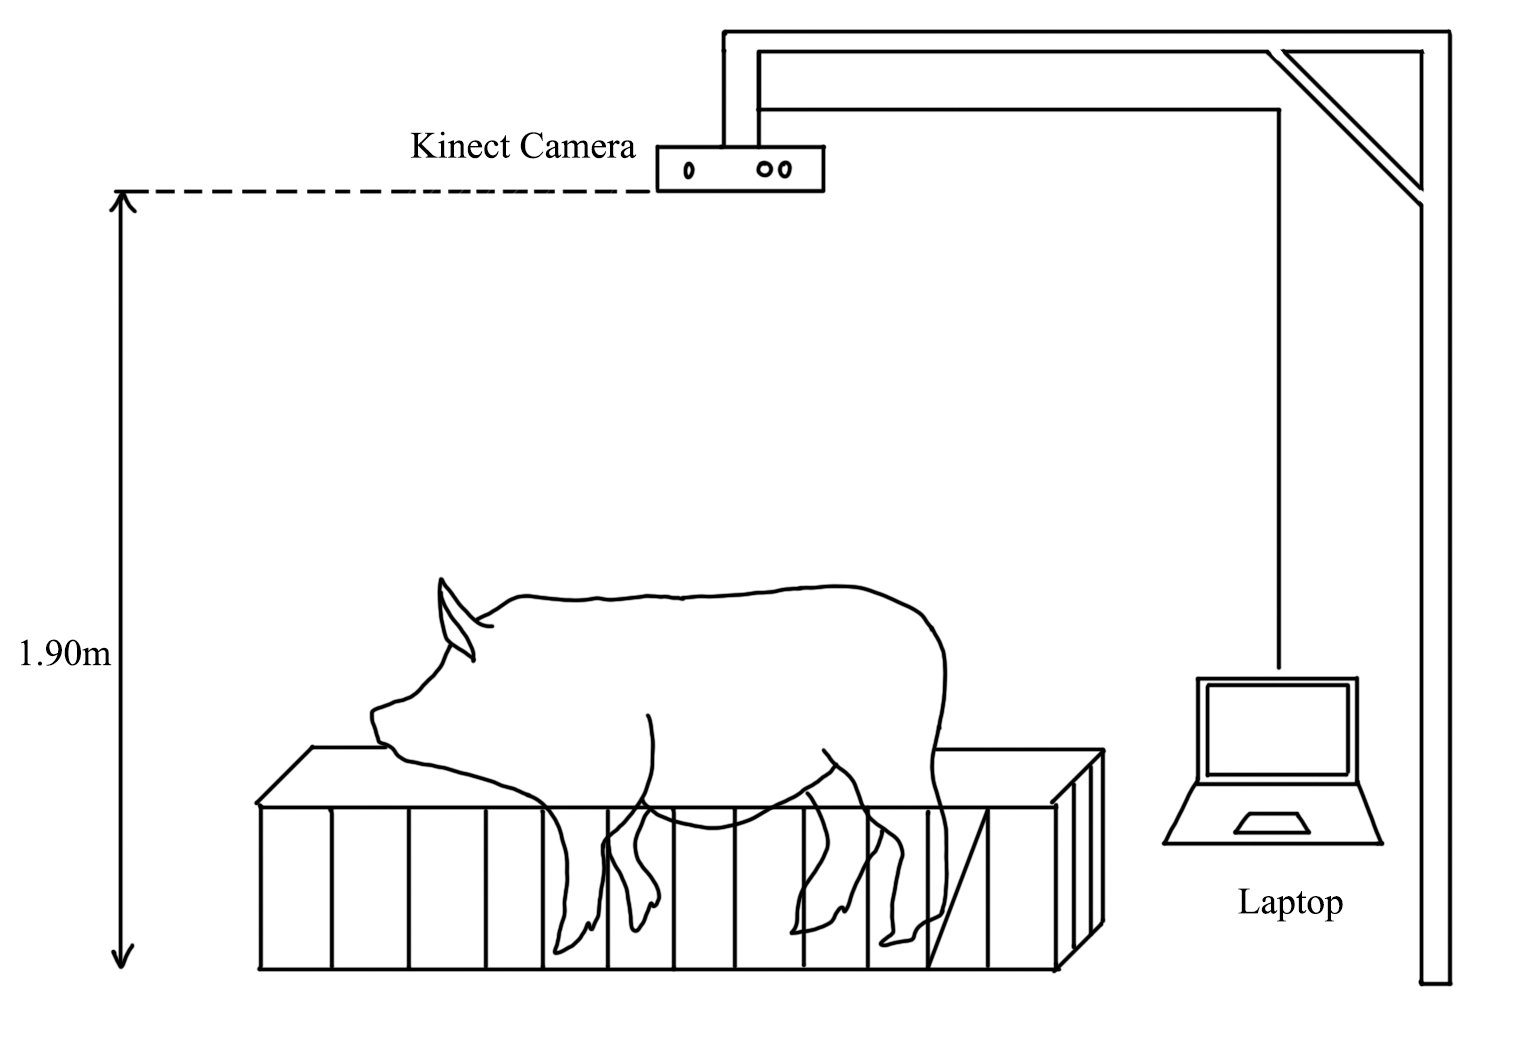
\includegraphics[height=0.4\textheight]{figures/pigpen_diagram}
	\caption{Pigpen Diagram}
	\label{fig:Pigpen Diagram}
\end{figure}

Figure 5 illustrates the pigpen setup, with the Microsoft Kinect V1 camera mounted 1.9 meters above the ground for a top-down view. This height ensures clear visibility of the pigs’ backs within the Kinect’s depth-sensing range (0.8–4.0 meters). The pigpen accommodates multiple pigs, with spacing to minimize occlusion, ensuring accurate volume estimation. The setup captures depth data for multiple pigs in a single frame while preserving individual measurements.

\newpage

\subsection{Camera Configuration}

\begin{figure}[h]
	\centering
	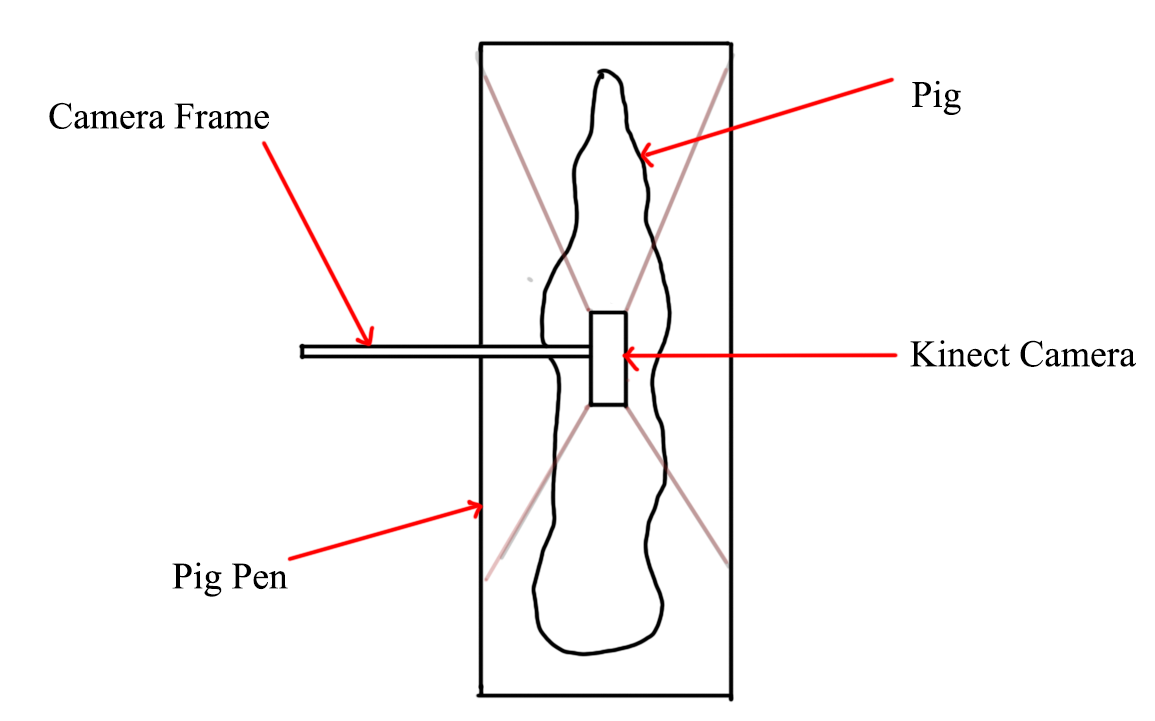
\includegraphics[height=0.4\textheight]{figures/Camera Setup 2}
	\caption{Camera Configuration}
	\label{fig:Camera Configuration}
\end{figure}

The Kinect V1 camera captured RGB and depth streams at 640$\times$480 pixels per video, side by side. The depth sensor was calibrated for its effective range, with the 1.9-meter height optimized for detailed body contour capture. A dedicated server processed and stored data in real time, ensuring minimal latency and high data integrity.

\section{Study Design and Data Collection}

The study was conducted in small, backyard-type pig farms in Cagayan de Oro City, Philippines, focusing on Landrace pigs, known for adaptability and rapid growth. The pigs, weighing 8–22 kilograms and aged 1–2 months, were raised under optimal conditions with high-protein diets, clean water, and regular health monitoring.

Depth data was collected using the Kinect V1 camera, positioned to capture a top-down view of the pigs’ backs, standardizing data collection. The system recorded RGB and depth streams simultaneously, as shown in \hyperref[fig:raw output]{Figure 7}. The RGB stream was processed by YOLOv11 for object detection, generating bounding boxes to localize pigs. These coordinates were mapped to the depth stream to extract corresponding depth data, ensuring accurate spatial and depth association.

Environmental variables, such as lighting and temperature, were controlled to maintain data quality. Poor lighting or extreme temperatures were avoided, and conditions were documented. Only pigs within the 8–22 kg range were included, with data captured when pigs were standing or in postures showing their backs clearly, optimizing volume estimation.

Features extracted included pixel size, non-zero pixel count, pixel-to-non-pixel ratio, standard deviation of depth, mean depth, pixel ratio, volume proxy, aspect ratio, perimeter \hyperref[Section 3.7]{(Section 3.7)}. These served as inputs for the hybrid LightGBM-CNN model. Processing and testing were conducted locally on a dedicated server for real-time feedback.

\subsection{Image Acquisition and Frame Selection}

The Microsoft Kinect V1 camera, mounted overhead at a height of 1.9 meters, was used to capture synchronized RGB and depth streams at 640$\times$480 resolution for each and 30 fps. To ensure high-quality data input, a manual quality assessment was performed. This filtering step selected frames that were sharp, well-lit, and free from motion blur—minimizing segmentation errors in multi-pig environments where occlusions are common.

\begin{figure}[h]
	\centering
	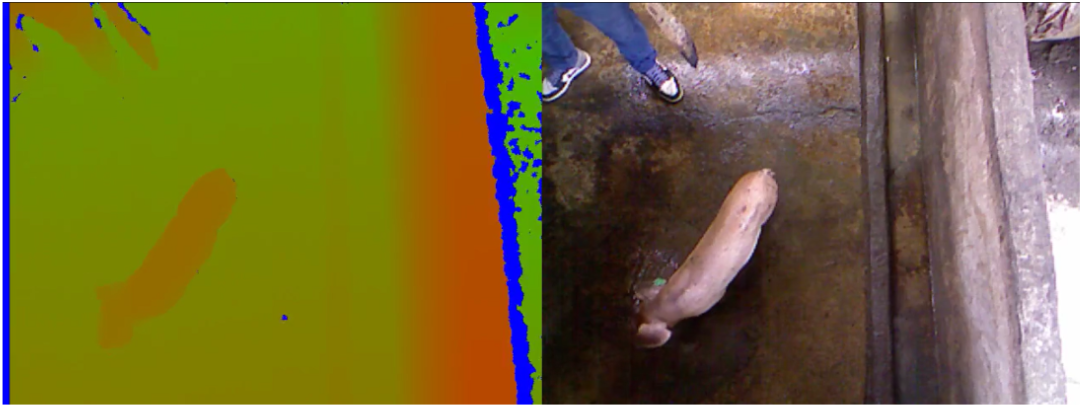
\includegraphics[height=0.25\textheight]{figures/Raw Data Collection}
	\caption{\textit{Raw Data Collection Output.} Screenshot from the Microsoft Kinect V1 video recording: RGB image on the right, depth image on the left. The camera is mounted overhead at 1.9 meters.}
	\label{fig:raw output}
\end{figure}

\newpage

\section{Object Detection}
Pigs were detected in the RGB frames using YOLOv11, a real-time object detection model fine-tuned on the DATA\_TONGHOP dataset\citep{khoi2024data_tonghop}. The resulting bounding box coordinates were then mapped to the corresponding depth frames to extract aligned regions of interest (ROIs).

\begin{figure}[h]
	\centering
	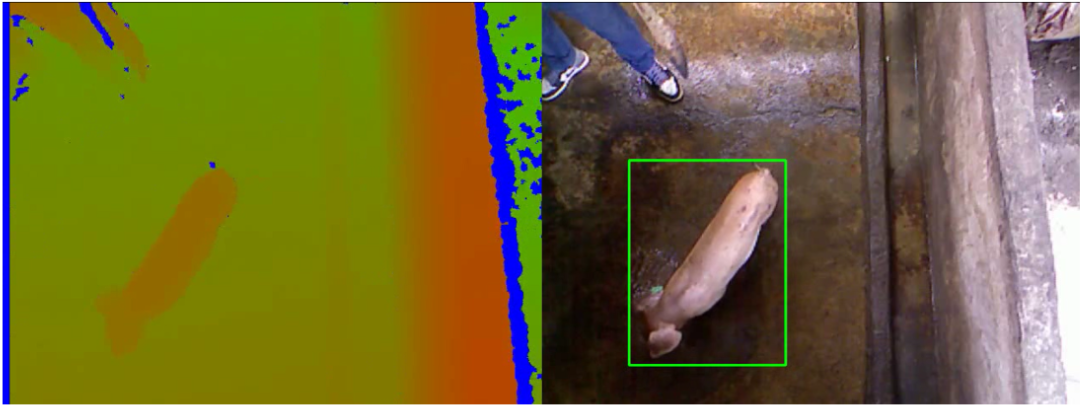
\includegraphics[height=0.25\textheight]{figures/Processed Video}
	\caption{\textit{Processed Video for Pig Detection.} The pig is detected in the RGB frame using the DATA\_TONGHOP dataset.}
	\label{fig:processed video}
\end{figure}

\begin{figure}[h]
	\centering
	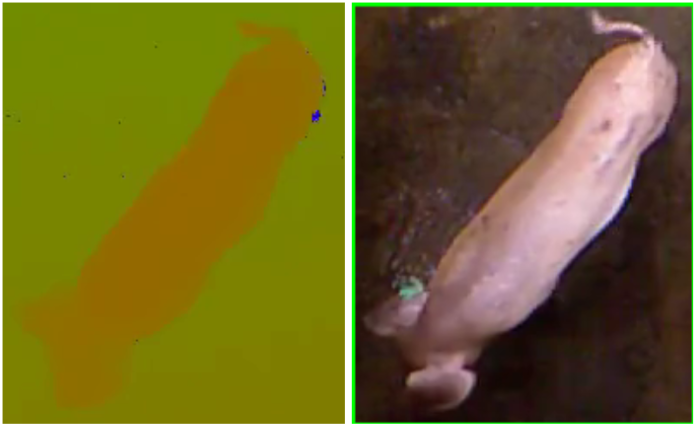
\includegraphics[height=0.25\textheight]{figures/Cropped images}
	\caption{\textit{Cropped images using bounding box coordinates.}}
	\label{fig:cropped images}
\end{figure}

\section{Segmentation Model}
The Segment Anything Model (SAM) was used for background removal and precise segmentation \citep{kirillov2023segment_anything}.SAM produced binary masks that removed background noise and retained only the pig region, improving the clarity and focus of the input. These masks were also used to extract pig-specific depth values.

\begin{figure}[h]
	\centering
	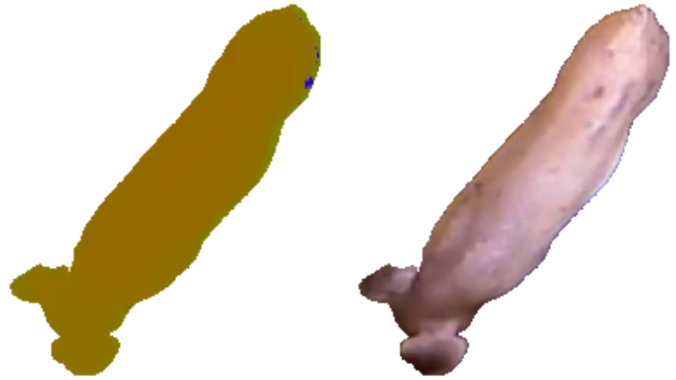
\includegraphics[height=0.25\textheight]{figures/Depth image segmentation}
	\caption{\textit{Depth image segmentation using RGB-based masking.} The RGB-detected pig mask was applied to the depth frame, isolating only the pig and discarding the background depth values.}
	\label{fig:Depth image segmentation}
\end{figure}

\section{Data Preprocessing}
Depth images collected from the Kinect V1 camera were preprocessed to enhance quality and consistency. The preprocessing pipeline included the following steps:

\begin{itemize}
	\item \textbf{Depth Normalization}: Depth values were normalized to a range of 0–255 using min-max scaling to standardize the input for the CNN model.
	\item \textbf{Contrast Enhancement}: A gamma correction ($\gamma$ = 1.2) was applied to improve the visibility of depth variations, aiding in feature extraction.
	\item \textbf{Data Augmentation}: To enhance model robustness and reduce overfitting, optional data augmentation techniques were applied during training, including:
	\begin{itemize}
		\item \textbf{Random Flipping}: Images were horizontally flipped with a 50\% probability to simulate variations in pig orientation.
		\item \textbf{Salt-and-Pepper Noise}: Random noise was introduced with varying probabilities (salt\_prob and pepper\_prob ranging from 0.02 to 0.10) to emulate sensor noise and environmental artifacts.
	\end{itemize}
\end{itemize}
The dataset was split into training and validation sets, stored in separate directories (train\_data and val\_data). Each directory contained subfolders for individual pigs, with depth images manually curated to ensure quality and relevance.

\section{Feature Extraction} \label{Section 3.7}

To accurately predict a pig’s weight using depth images captured from a Microsoft Kinect V1 sensor, a comprehensive set of features was extracted from each segmented image. These features were designed to capture both geometric and depth-related characteristics of the pig’s body as observed in the top-down view provided by the depth camera. The extracted features were used as inputs for the hybrid CN-LGBM model, combining Convolutional Neural Networks (CNN) and Light Gradient Boosting Machine (LightGBM). Each feature was chosen based on its relevance to shape, size, volume, or surface variation, all of which are strongly correlated with body mass.

The extracted features included the following:
\begin{longtable}{| >{\centering\arraybackslash}m{0.15\linewidth} | >{\centering\arraybackslash}m{0.25\linewidth} | m{0.50\linewidth} |}
	\caption{Extracted Features}
	\label{tab:extracted features}\\
	\hline
	\textbf{Feature} & \textbf{Description} & \textbf{Equation} \\
	\hline
	Pixel Size
	& 
	Total number of pixels in the segmented region (height $\times$ width). 
	&
	\begin{equation}
		Pixel \; Size = h \times w
	\end{equation}
	\myequation{Pixel Size}
	\\
	\hline
	Non-Zero Pixel Count
	& 
	Count of valid (non-zero) depth pixels, excluding background or occluded areas.
	&
	\begin{equation}
		Non-Zero \; Count = \sum(D>0)
	\end{equation}
	\myequation{Non-Zero Pixel Count}
	\\
	\hline
	Pixel-to-Non-Pixel Ratio
	& 
	Proportion of valid pixels to total pixels in the segmented region.
	&
	\begin{equation}
		Ratio = \frac{Non-Zero \; Count}{Pixel \; Size}
	\end{equation}
	\myequation{Pixel-to-Non-Pixel Ratio}
	\\
	\hline
	Standard Deviation of Depth
	& 
	Measures variability in depth values across valid pixels.
	&
	\begin{equation}
		\sigma = \sqrt{\frac{1}{n}\sum_{i=1}^{n}(x_i - \bar{x})^2}
	\end{equation}
	\myequation{Standard Deviation of Depth}
	\\
	\hline
	Mean Depth
	& 
	Average depth value across non-zero pixels. 
	&
	\begin{equation}
		\mu = \frac{1}{n}\sum_{i=1}^{n}x_i \quad where \; x_i > 0
	\end{equation}
	\myequation{Mean Depth}
	\\
	\hline
	Pixel Ratio
	& 
	Ratio of valid pixels to the entire image resolution.
	&
	\begin{equation}
		Pixel \; Ratio = \frac{Non-Zero \; Count}{1280\times480}
	\end{equation}
	\myequation{Pixel Ratio}
	\\
	\hline
	Volume Proxy
	& 
	Sum of all valid depth values; proxy for body volume.
	&
	\begin{equation}
		Volume \; Proxy = \sum D
	\end{equation}
	\myequation{Volume Proxy}
	\\
	\hline
	Aspect Ratio
	& 
	Width-to-height ratio of the pig’s bounding box.
	&
	\begin{equation}
		Aspect \; Ratio = \frac{w}{h}
	\end{equation}
	\myequation{Aspect Ratio}
	\\
	\hline
	Perimeter
	& 
	Total length around the segmented contour.
	&
	\begin{multline}
		Perimeter = \\ 
		\sum arcLength (C_i , closed=True)
	\end{multline}
	\myequation{Perimeter}
	\\
	\hline
\end{longtable}

All features were normalized using min-max scaling:
\begin{equation}
	x_{normalized} = \frac{(x - min(x))}{(max(x) - min(x) + 1e-8)}
\end{equation}
\myequation{Min-Max Normalization}

This normalization ensures that feature values are within a uniform range [0, 1], which improves model convergence and performance in both CNN and LightGBM architectures. Additionally, sectional volumes were computed by dividing the segmented region into smaller subregions, allowing for a more localized analysis of body mass distribution.

These features collectively provide a rich and multi-dimensional input representation of each pig’s physical characteristics, enabling the CN-LGBM model to effectively learn patterns correlated with body weight.


\section{Model Training}
A hybrid LightGBM-CNN model was developed to leverage tabular features and spatial information for weight estimation, implemented using LightGBM and PyTorch.

\newpage

\subsection{Model Architecture}

\begin{figure}[h]
	\centering
	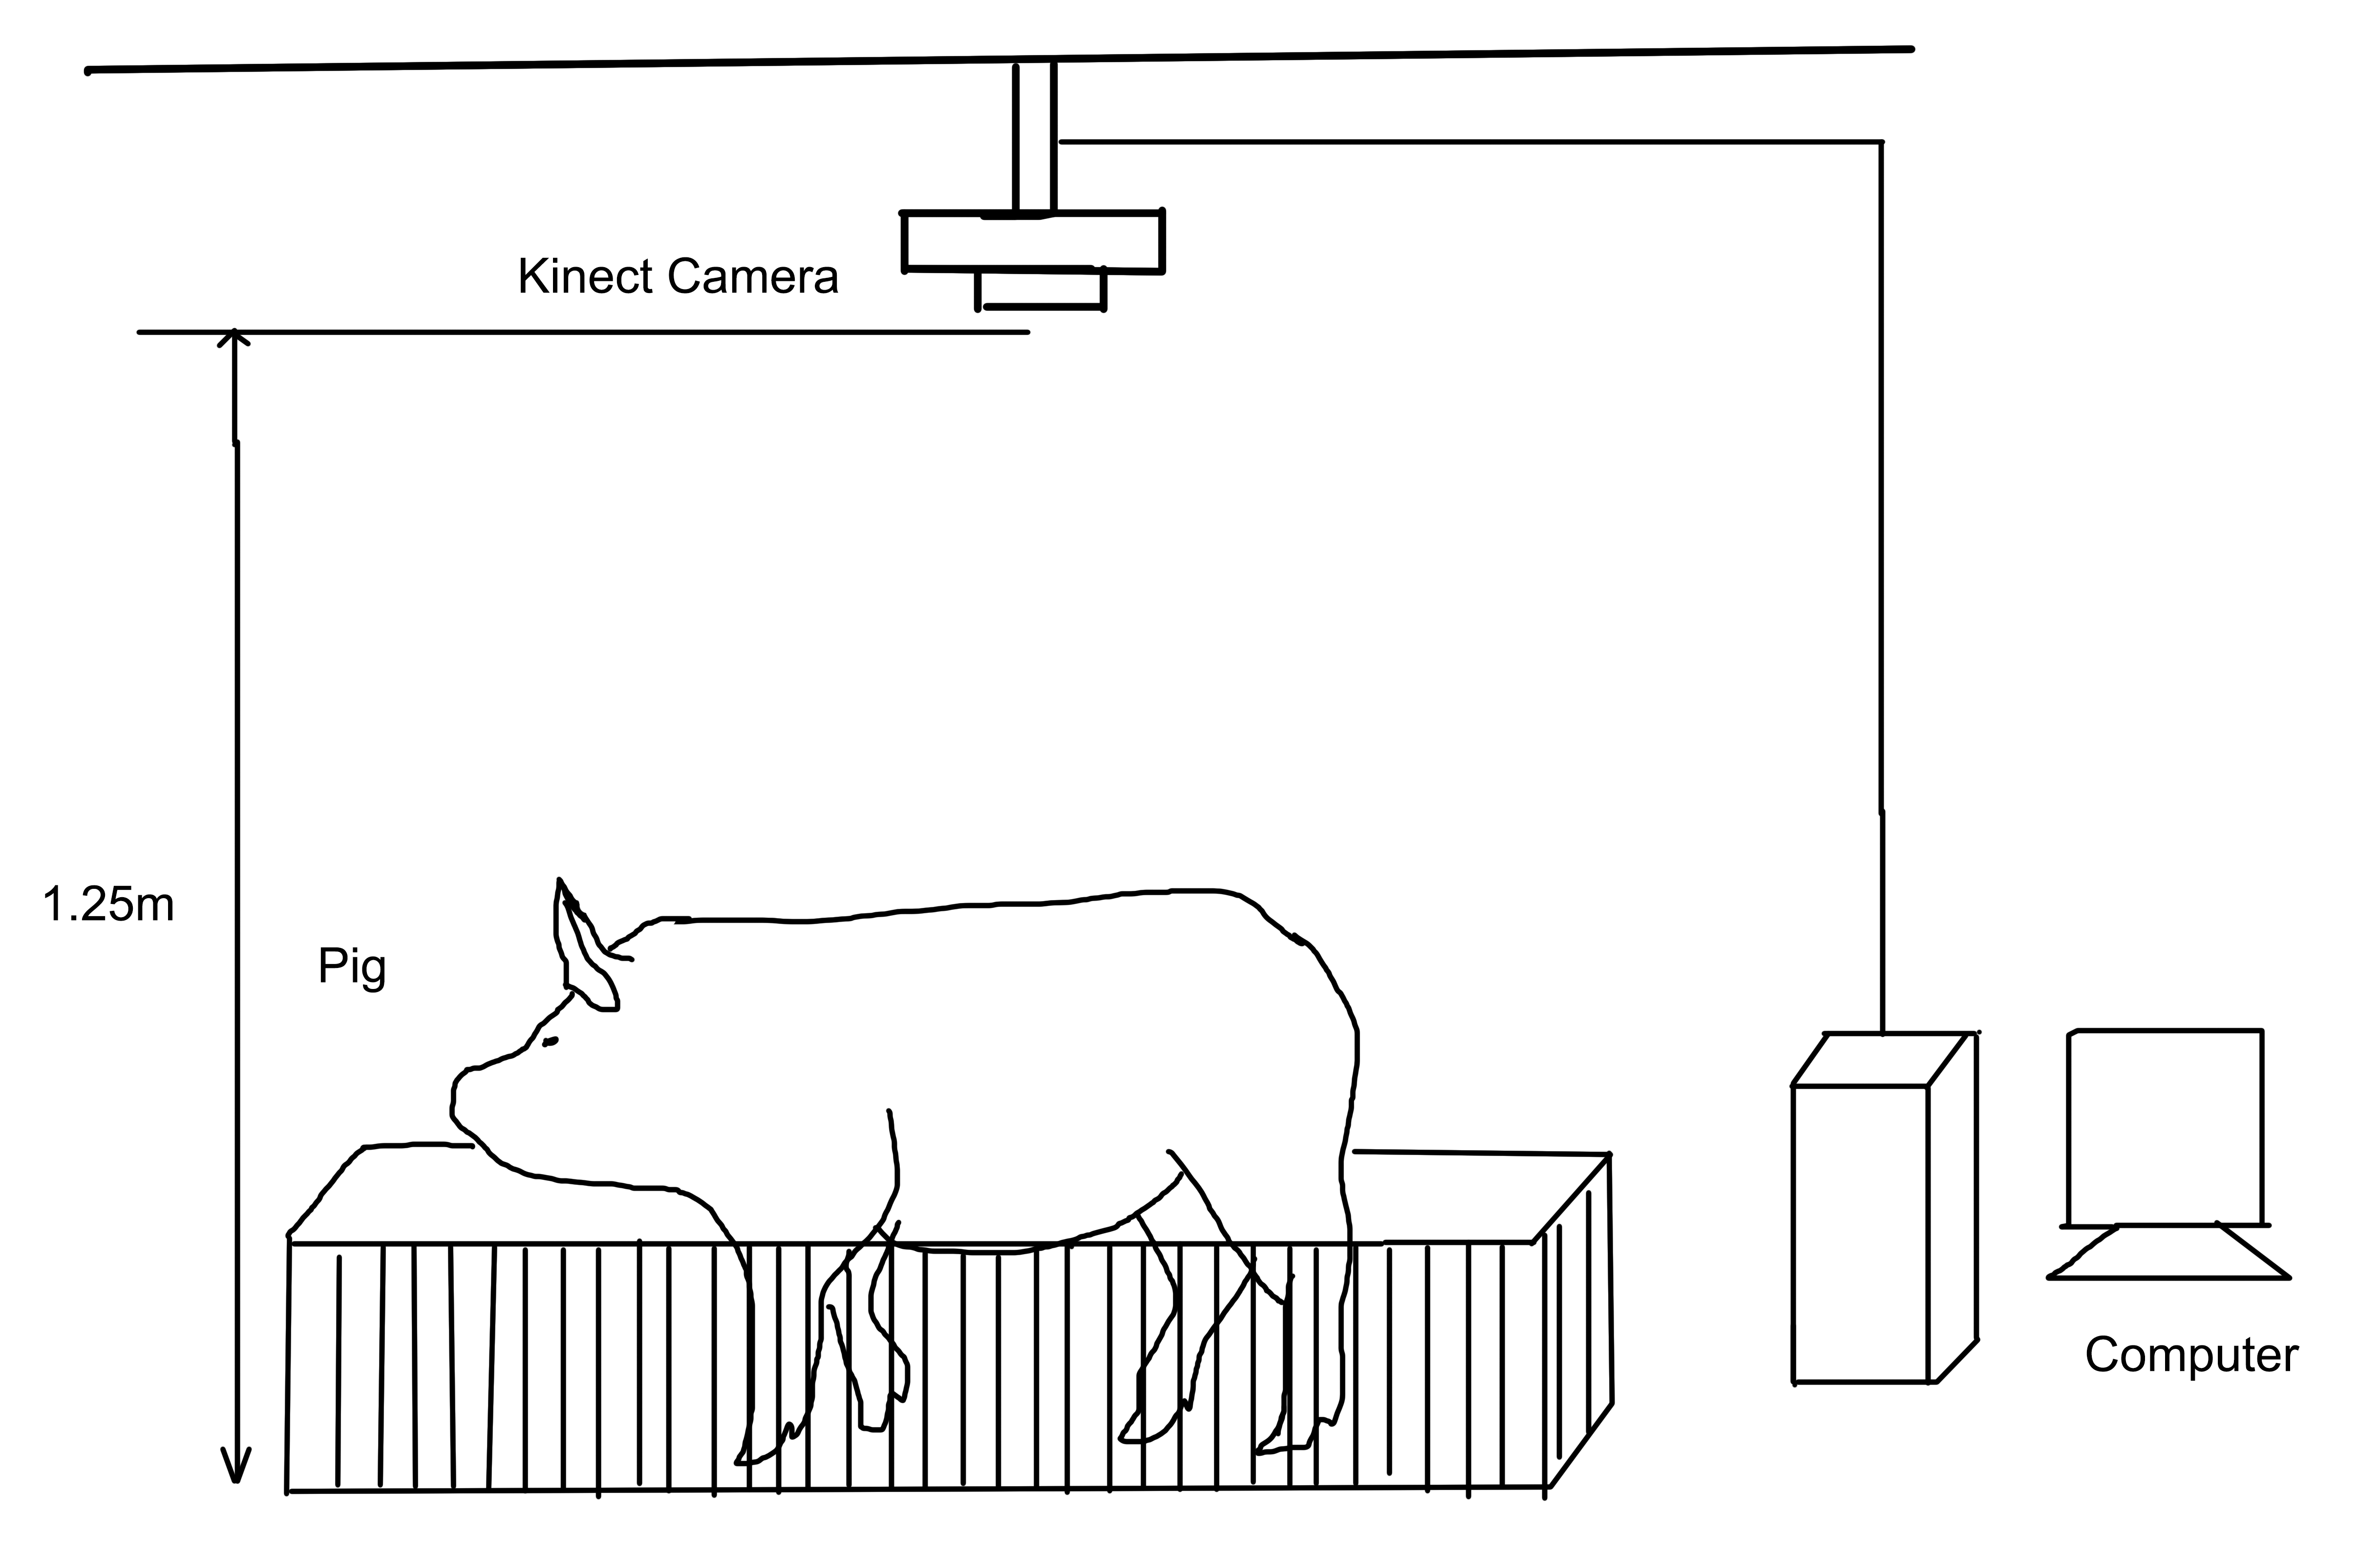
\includegraphics[height=0.4\textheight]{figures/Untitled-1wqw}
	\caption{Model Architecture}
	\label{fig:Model Architecture}
\end{figure}

\noindent \textbf{LightGBM Model}

The LightGBM regressor was trained on the 9 features (pixel size, non-zero pixel count, pixel-to-non-pixel ratio, standard deviation of depth, mean depth, pixel ratio, volume proxy, aspect ratio, and perimeter to provide an initial weight prediction. The training dataset was split into 80\% training and 20\% validation sets using a random seed for reproducibility. It used default hyperparameters (e.g., 100 trees, learning rate 0.1) and was saved as lgbm\_model.pkl. The model provided an initial weight prediction, evaluated using root mean square error (RMSE).
\\
\\
\noindent \textbf{CNN Model}

The CNN refined predictions using depth images and the LightGBM prediction. The architecture included:
\begin{itemize}
	\item \textbf{Convolutional Layers}: Three layers with 32, 64, and 128 channels, respectively, each using 3$\times$3 kernels, ReLU activation, and max-pooling with a 2$\times$2 kernel and stride 2.
	\item \textbf{Fully Connected Layers}: Three layers with 512, 256, and 1 neurons, respectively, using ReLU activation for the first two layers and linear activation for the output layer.
	\item \textbf{Input Integration}: The CNN processes depth images (1 channel, 256$\times$384 for training, 40$\times$80 for deployment) and integrates the LightGBM prediction, concatenated with flattened CNN features before the first fully connected layer.
\end{itemize}

\noindent \textbf{Hybrid Integration}

The LightGBM prediction was fed into the CNN as an additional feature, enhancing the model’s ability to combine tabular and spatial data. The final output was a single weight estimate in kilograms.

\subsection{Training Procedure}

The dataset was split into 80\% training (4,000 samples) and 20\% validation (1,000 samples) sets using a random seed. The training process involved:
\begin{itemize}
	\item \textbf{LightGBM Training}: Trained on the 9 features using default hyperparameters.
	\item \textbf{CNN Training}: Trained for 15 epochs using the Adam optimizer (learning rate 0.002) and mean squared error (MSE) loss. Depth images were resized to 256$\times$384 and normalized. The LightGBM predictions were concatenated with CNN features. Training and validation losses were plotted to monitor convergence and detect overfitting.
	\item \textbf{Hybrid Training}: The CNN was fine-tuned with the LightGBM predictions, optimizing the combined model. The best model, based on the lowest validation loss, was saved.
\end{itemize}

\section{Model Evaluation} \label{Section 3.9}
The hybrid model was evaluated on the test set (1,000 samples) using:
\begin{itemize}
	\item \textbf{Mean Absolute Error (MAE)}: Average absolute difference between predicted and actual values, measured in kilograms (kg).
	\item \textbf{Root Mean Squared Error (RMSE)}: Square root of the average of squared differences between predicted and actual values.
\end{itemize}

The model achieved an MAE of 0.38 kg and an RMSE of 0.52 kg indicating high accuracy. Five-fold cross-validation yielded an average MAE of 0.40 kg. The hybrid model outperformed standalone LightGBM (RMSE ~0.65 kg) and CNN (RMSE ~0.60 kg) models. Manual review confirmed prediction alignment with pig size and posture.

\section{Model Deployment} \label{Section 3.10}
To enable practical use in agricultural settings, a deployment pipeline was developed using a FastAPI-based web service, ensuring seamless interaction with the hybrid model for weight prediction.

\subsection{Deployment Architecture}

The deployment system used FastAPI to create a RESTful API for weight prediction, accepting depth images and features, processing them through the LightGBM and CNN models, and returning predicted weights. The system is lightweight, scalable, and accessible via HTTP requests, suitable for farm management systems or mobile applications. Components included:

\begin{itemize}
	\item \textbf{LightGBM Model}: Provides initial predictions based on the 9 features.
	\item \textbf{CNN Model}: Refines predictions using preprocessed depth images.
	\item \textbf{FastAPI Server}: Handles requests, validates inputs, and orchestrates predictions.
\end{itemize}

The models were deployed on a server with GPU support for CNN inference, with CPU fallback for compatibility. The server was tested locally but can be hosted on cloud platforms.

\begin{figure}[h]
	\centering
	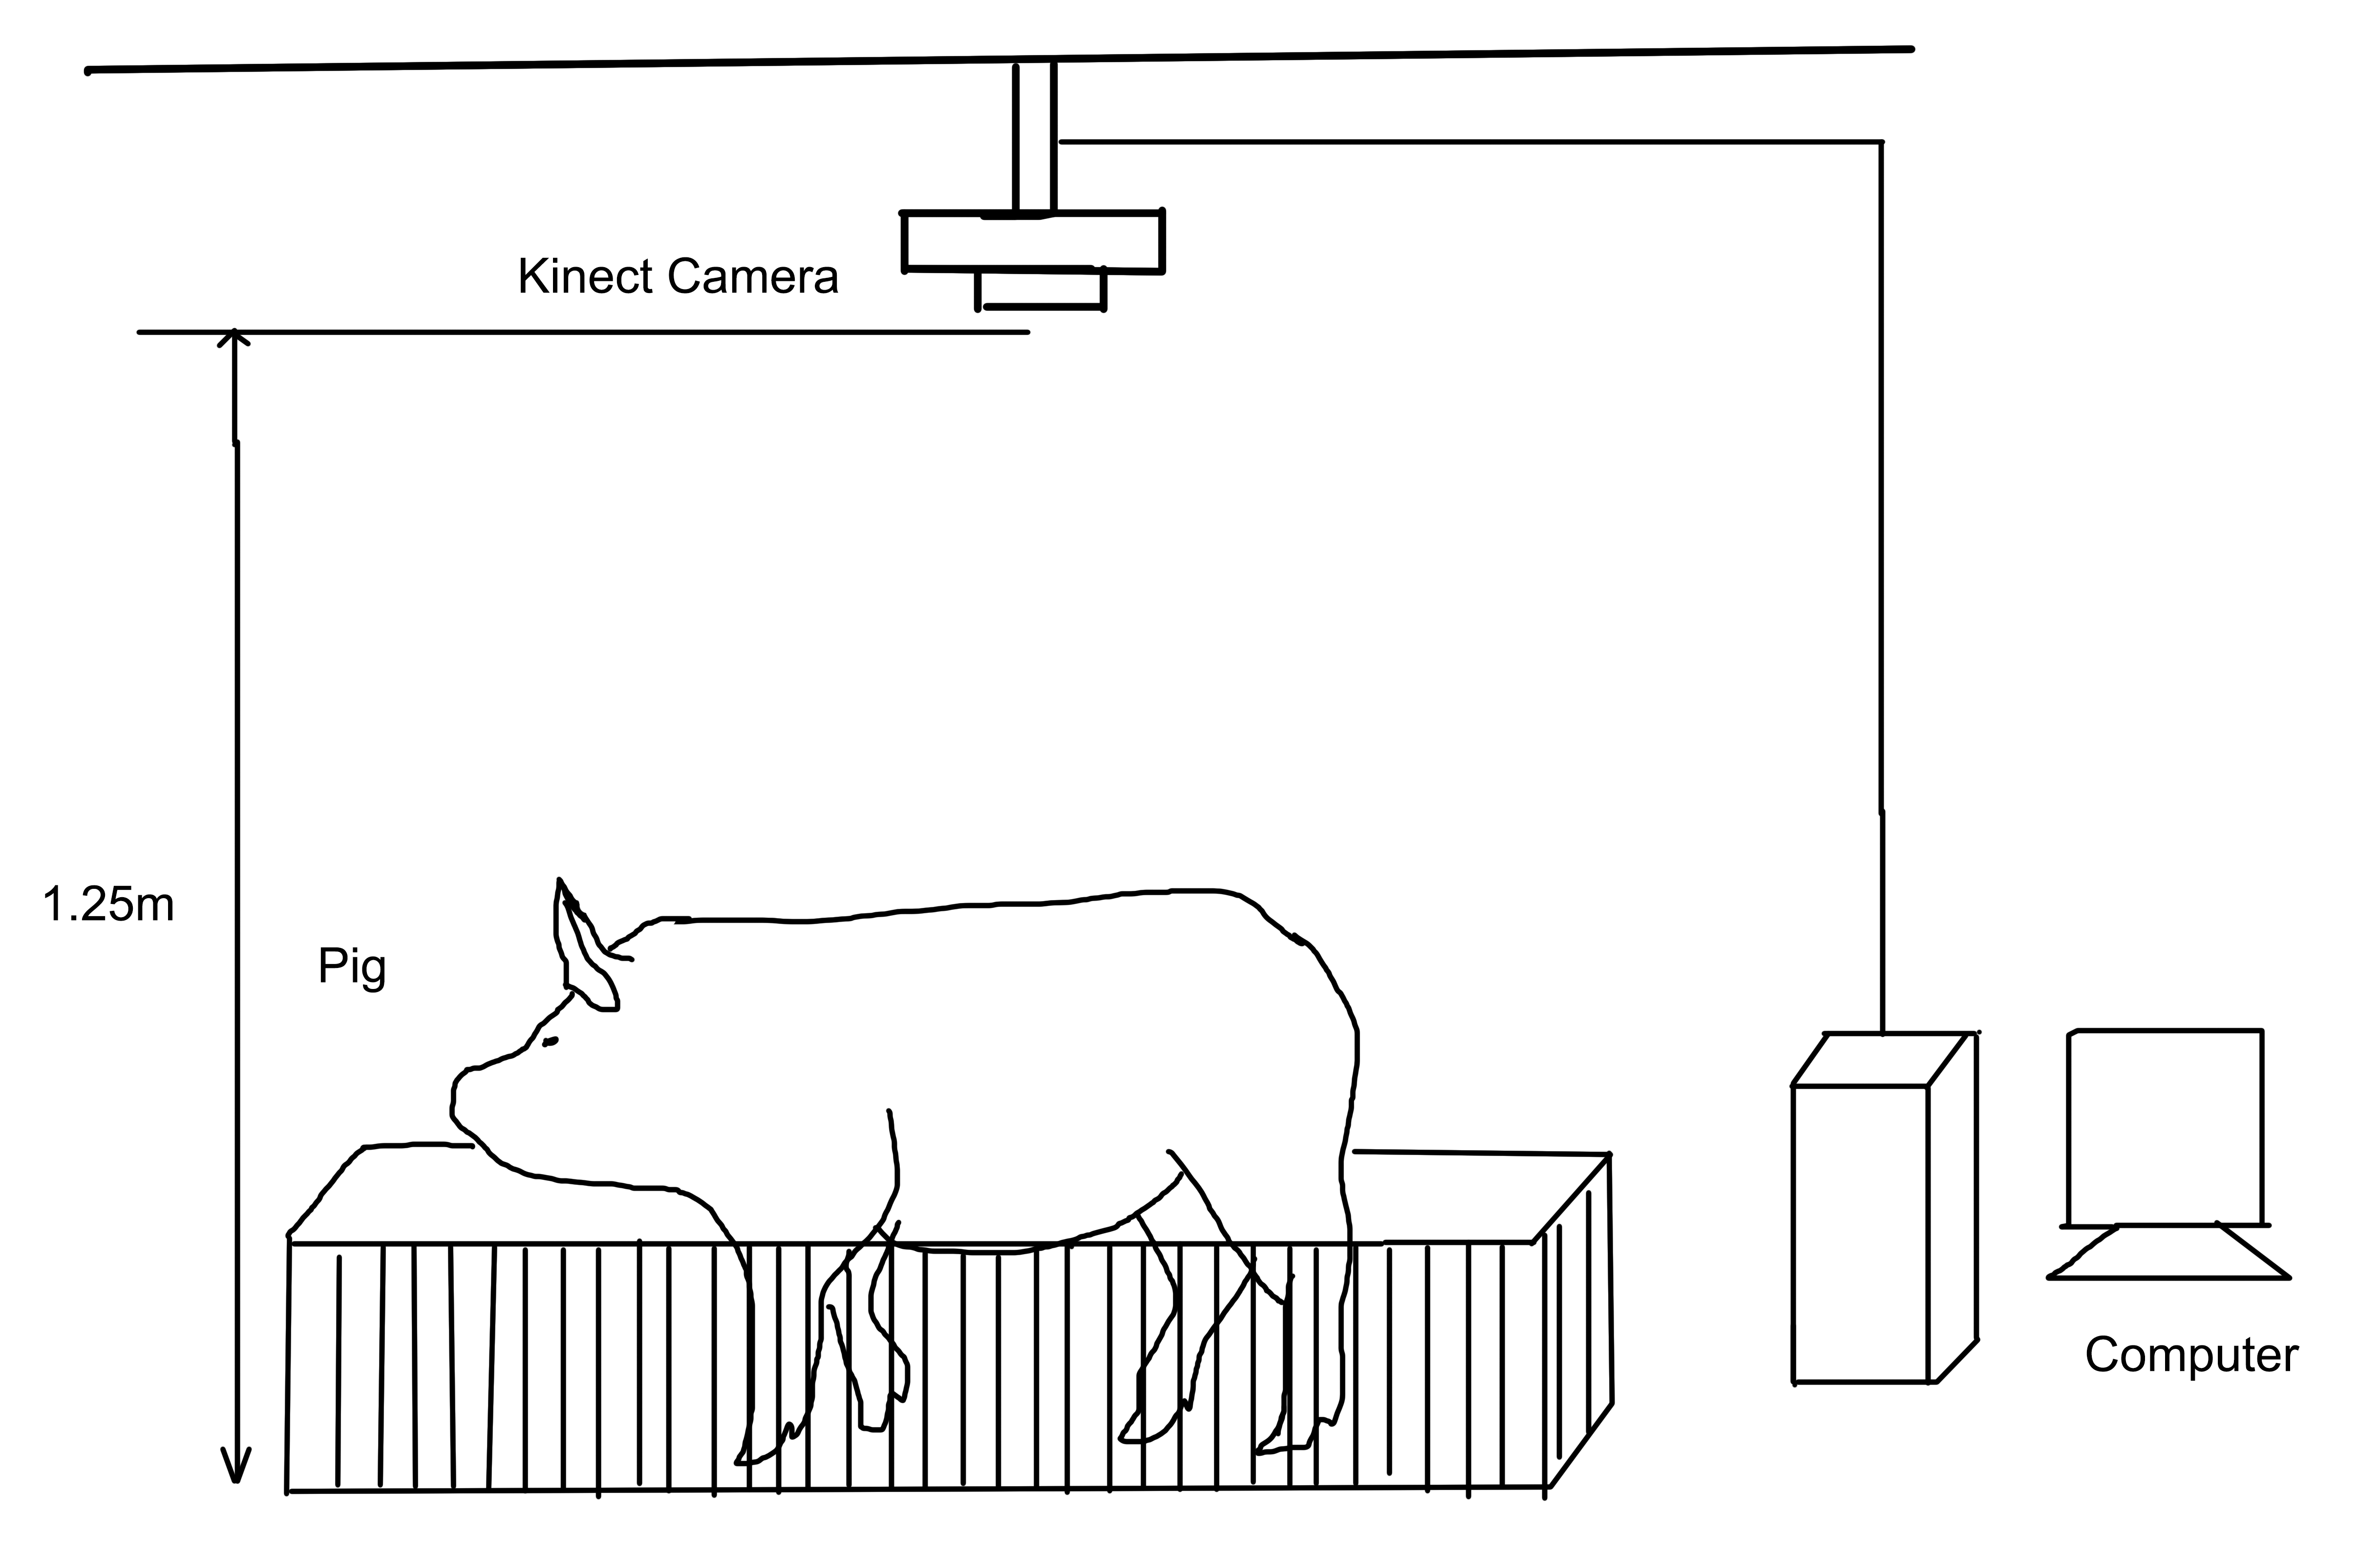
\includegraphics[height=0.4\textheight]{figures/Untitled-1wqw}
	\caption{Deployment Architecture}
	\label{fig:Deployment Architecture}
\end{figure}

\subsection{Model Loading and Configuration}

\begin{itemize}
	\item \textbf{LightGBM Model}: Loaded from $lgbm\_model.pkl$ using the pickle library, processing tabular features.
	\item \textbf{CNN Model}: Loaded from $model\_1745138618.8710697.pt$ using PyTorch, set to evaluation mode $(model.eval())$. The model ran on GPU or CPU based on $torch.cuda.is\_available()$.
\end{itemize}

Error handling managed issues like missing model files or incompatible architectures.

\subsection{Input Preprocessing}

The API accepts depth images (PNG/JPEG) and optional features:

\begin{itemize}
	\item \textbf{Image Preprocessing}:
	\begin{itemize}
		\item Convert to grayscale, threshold low-intensity pixels ($\leq$1 set to 0).
		\item Resize to 40$\times$80 pixels using linear interpolation.
		\item Normalize depth values to [0, 255], then [0, 1].
		\item Convert to PyTorch tensor (1, 1, 40, 80).
	\end{itemize}
	\item \textbf{Feature Processing}:
	\begin{itemize}
		\item Accept features as JSON or Pydantic model (FeatureInput).
		\item Default to zeros if features are missing.
		\item Reshape features into a 1$\times$9 array for LightGBM.	
	\end{itemize}
\end{itemize}

\subsection{API Endpoint and Functionality}

\begin{itemize}
	\item \textbf{Root Endpoint (GET /)}: Returns {"message": "Weight Prediction API is running"}.
	\item \textbf{Prediction Endpoint (POST /predict/)}:
	\begin{itemize}
		\item \textbf{Inputs}: Depth image file, optional features (JSON/Pydantic).
		\item \textbf{Processing}: Validate image, preprocess, pass to CNN; validate features, pass to LightGBM; concatenate LightGBM prediction with CNN features for final prediction.
		\item \textbf{Output} JSON response {"predicted\_weight": value}.
		\item \textbf{Error Handling}: Manages invalid inputs and server issues with appropriate HTTP status codes.
	\end{itemize}
\end{itemize}

\subsection{Integration with Data Collection Pipeline}

The API integrates with the data collection pipeline \hyperref[Section 3.1]{(Sections 3.1–3.4)}. Depth images from the Kinect V1 and features from YOLOv11/SAM processing are sent to the API for real-time weight estimation, assuming proper camera positioning and pig visibility.

\section{Web Application for Real-Time Weight Estimation}
A web application was developed to interface with the Kinect V1 and FastAPI API, enabling real-time weight estimation for farmers.

\subsection{Web Application System Architecture}

The client-server system included:

\begin{itemize}
	\item \textbf{Client-Side Interface}: Browser-based front-end using React for a user-friendly interface to initiate capture, view streams, and display weights.
	\item \textbf{Kinect V1 Integration}: Local server process capturing RGB and depth streams.
	\item \textbf{FastAPI Backend}: Handles prediction requests \hyperref[Section 3.10]{(Section 3.10)}.
	\item \textbf{Communication Layer}: WebSocket/HTTP for real-time data transfer.
\end{itemize}

The system was optimized for low-latency performance.

\begin{figure}[h]
	\centering
	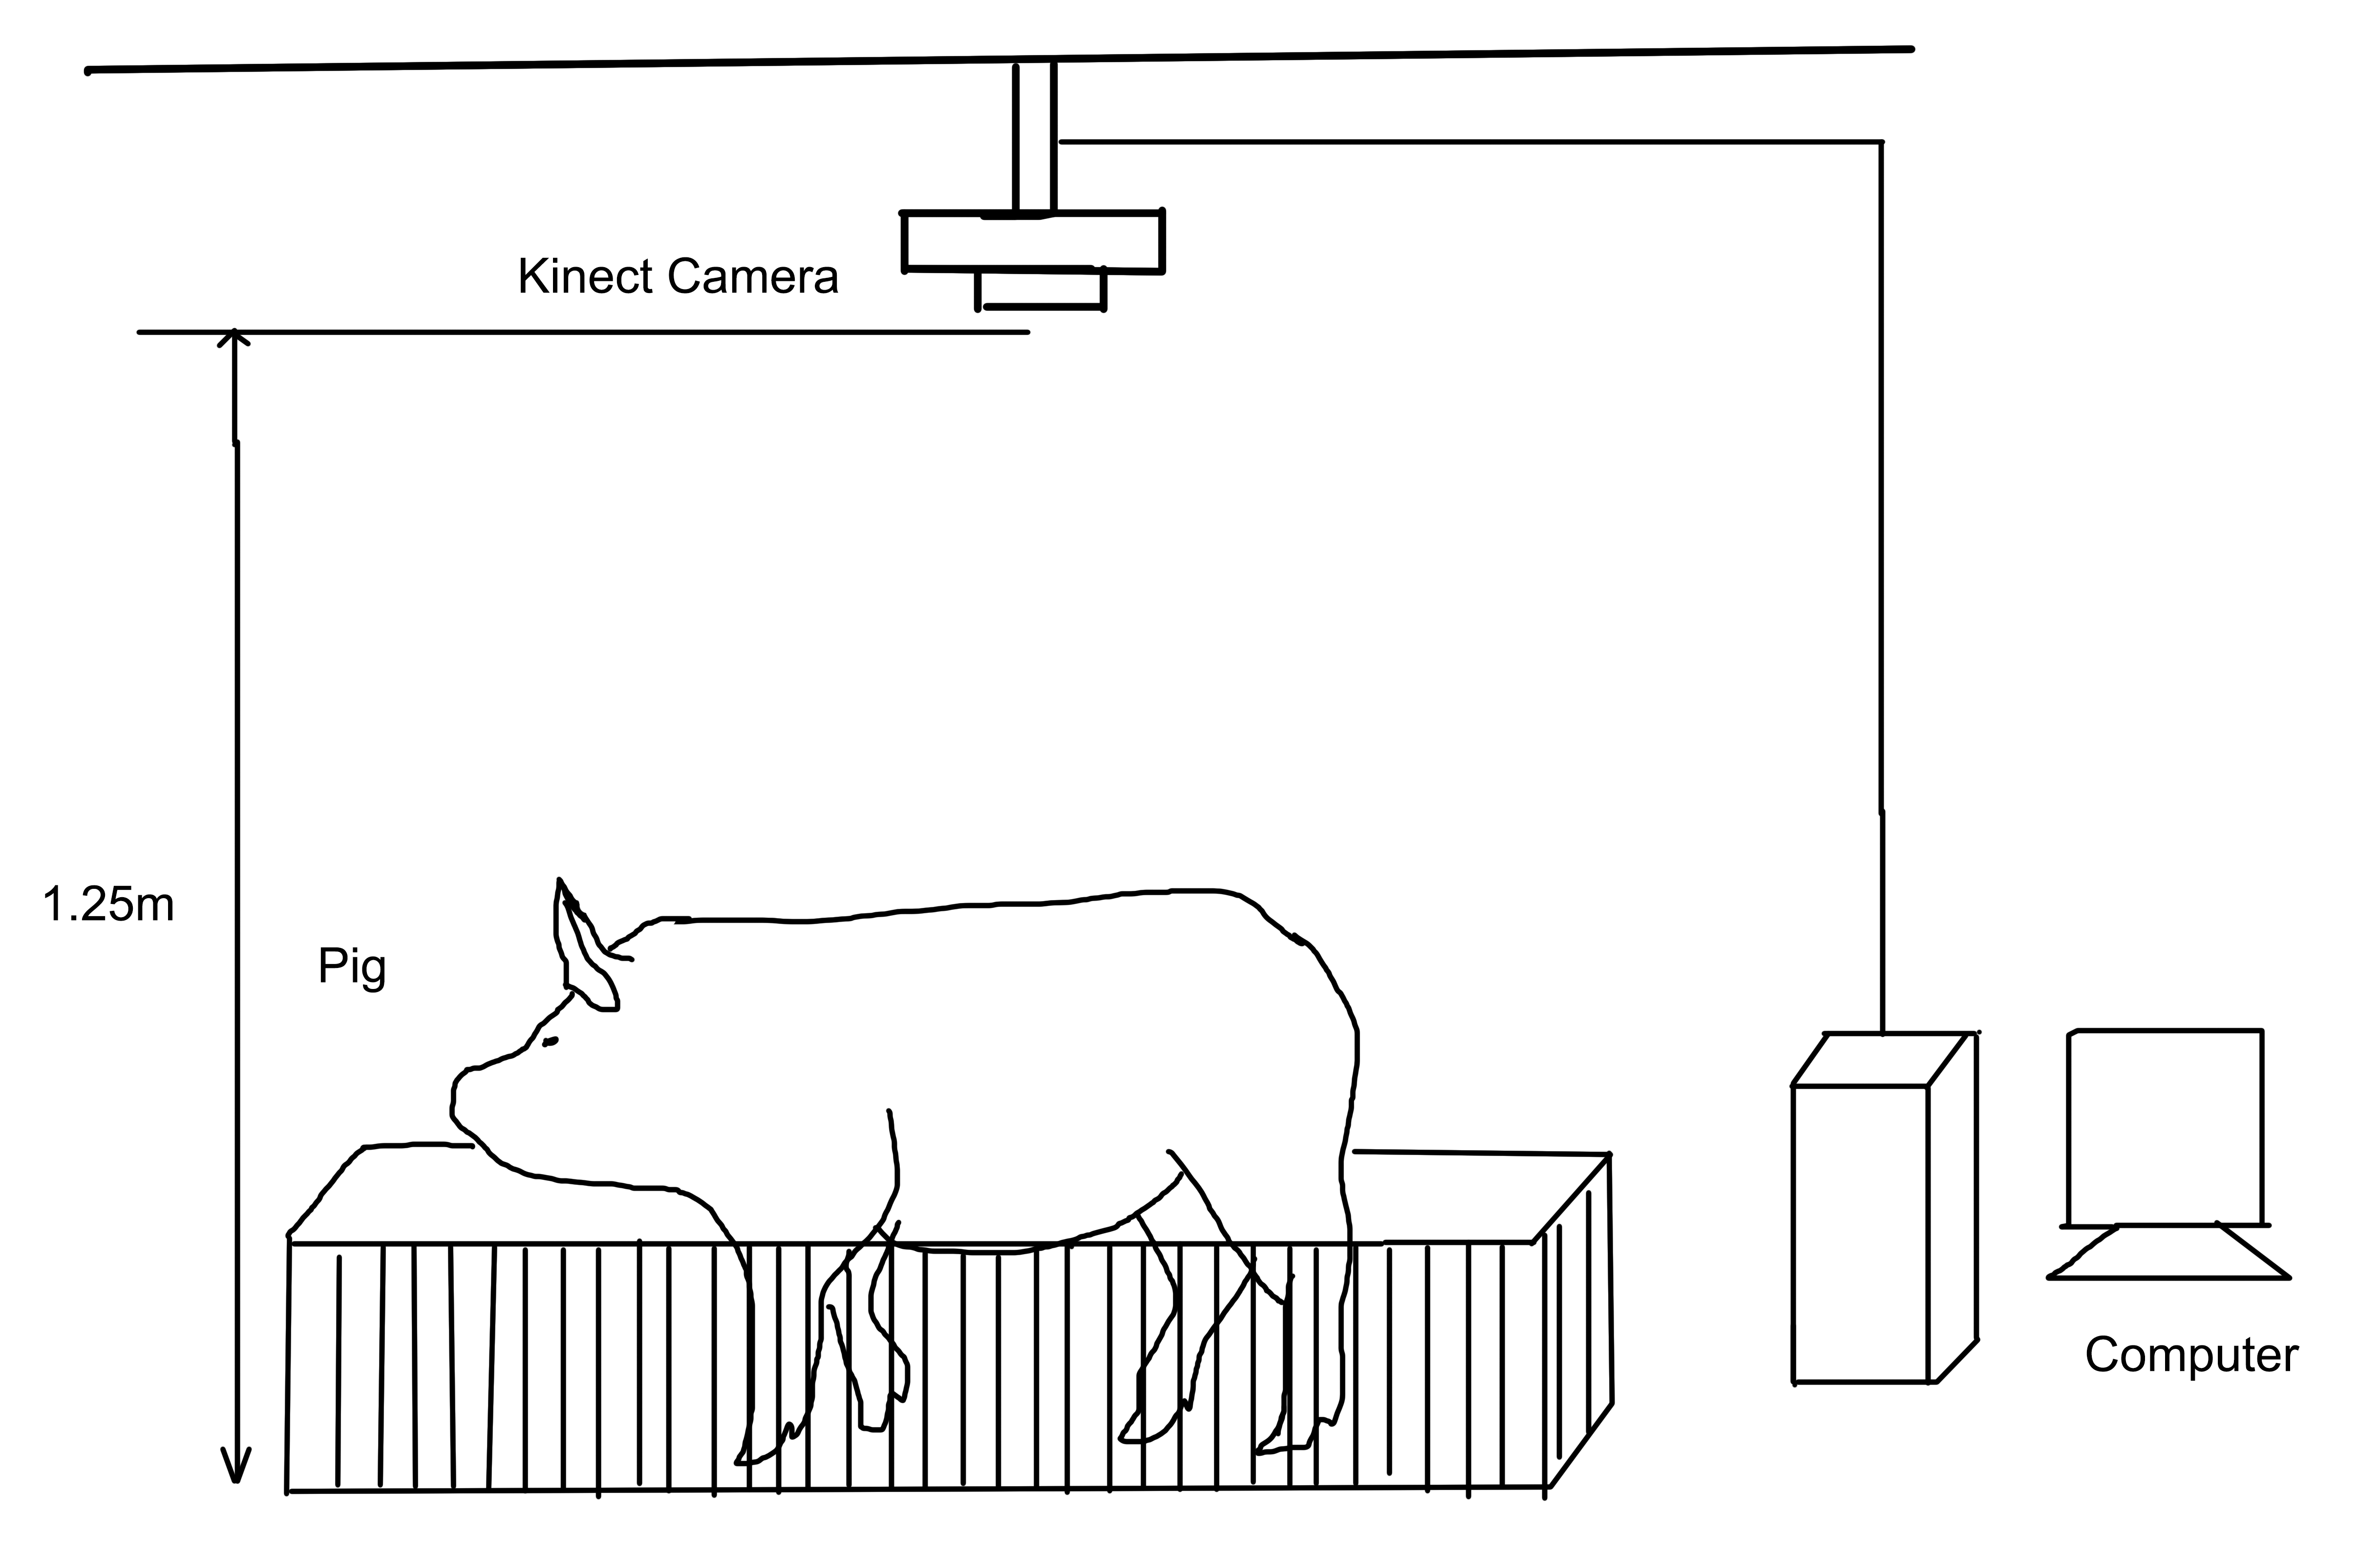
\includegraphics[height=0.4\textheight]{figures/Untitled-1wqw}
	\caption{System Architecture}
	\label{fig:System Architecture2}
\end{figure}

\newpage

\subsection{Kinect V1 Camera Integration}

The Kinect V1, mounted at 1.9 meters, captured depth and RGB streams at 640×480 pixels, 30 fps:

\begin{itemize}
	\item \textbf{Driver and SDK}: Microsoft Kinect SDK (v1.8) on a Windows computer.
	\item \textbf{Real-Time Capture}: Python script using pykinect/OpenKinect captured synchronized streams, prioritizing depth data.
	\item \textbf{Preprocessing}: Depth frames were thresholded ($\leq$1 set to 0), resized to 40$/times$80, and normalized to [0, 255].
\end{itemize}

\subsection{Web Application Development}

The React-based application featured:

\begin{itemize}
	\item \textbf{Live Video Feed}: Displays Kinect RGB stream via WebSocket/MJPEG.
	\item \textbf{Capture Trigger}: Manual or automated (via YOLOv11) to capture frames with clear pigs.
	\item \textbf{Prediction Display}: Dashboard showing predicted weights and confidence indicators.
\end{itemize}

The back-end handled camera communication and forwarded data to the FastAPI server.

\subsection{Real-Time Processing Pipeline}

\begin{itemize}
	\item \textbf{Frame Capture}: Kinect V1 captures synchronized frames.
	\item \textbf{Object Detection}: YOLOv11 detects pigs, generating bounding boxes.
	\item \textbf{Segmentation}: SAM isolates pigs in depth frames.
	\item \textbf{Feature Extraction}: Computes 9 features.
	\item \textbf{Prediction Request}: Sends data to FastAPI /predict/ endpoint.
	\item \textbf{Result Display}: Shows predicted weight on the interface.
\end{itemize}

The pipeline processed high-quality frames to minimize latency.

\subsection{Deployment and Testing}

Deployed locally on a Windows computer with the Kinect V1, tested in Cagayan de Oro City:

\begin{itemize}
	\item \textbf{Environmental Control}: Monitored lighting and temperature.
	\item \textbf{Camera Positioning}: Verified at 1.9 meters.
	\item \textbf{Performance}: Evaluated latency and accuracy against manual measurements.
\end{itemize}

The system is lightweight and can be containerized for cloud deployment.

\section{Data Processing Pipeline}

The Kinect sensor will be mounted in a fixed position above the pigpen to capture real-time The pipeline included:

\begin{enumerate}
	\item \textbf{Data Acquisition}: Kinect V1 captures RGB and depth streams.
	\item \textbf{Object Detection}: YOLOv11 generates bounding boxes.
	\item \textbf{Segmentation}: SAM isolates pigs.
	\item \textbf{Advanced Processing}: Contour detection, PCA alignment, valley detection.
	\item \textbf{Feature Extraction}: Compute 9 features.
	\item \textbf{Preprocessing}: Normalize, filter, augment data.
	\item \textbf{Training}: Train hybrid LightGBM-CNN model.
	\item \textbf{Evaluation}: Assess with MAE, RMSE, R².
	\item \textbf{Deployment}: FastAPI API for predictions.
	\item \textbf{Web Application}: Real-time estimation interface.
\end{enumerate}

The pipeline was implemented in Python, with the Jupyter notebook (Appendix A) providing the code.

\section{Ethical Considerations}

Non-invasive data collection adhered to animal welfare standards. Minimal disturbance was ensured, and ethical approval was obtained.

\section{Limitations}

The Kinect V1’s depth resolution may be affected by environmental factors. The focus on Landrace pigs (8–22 kg) limits generalizability. Errors in detection, segmentation, or feature extraction could impact accuracy.